% \vspace{0.75\baselineskip} 
% \rule{\textwidth}{0.4pt}\vspace*{-\baselineskip}\vspace{3.2pt}
% \rule{\textwidth}{1.6pt}
% \vspace{2\baselineskip}
\section{Options flowchart and explanation~\ref{fig:options}}
\begin{figure}
    \centering 
    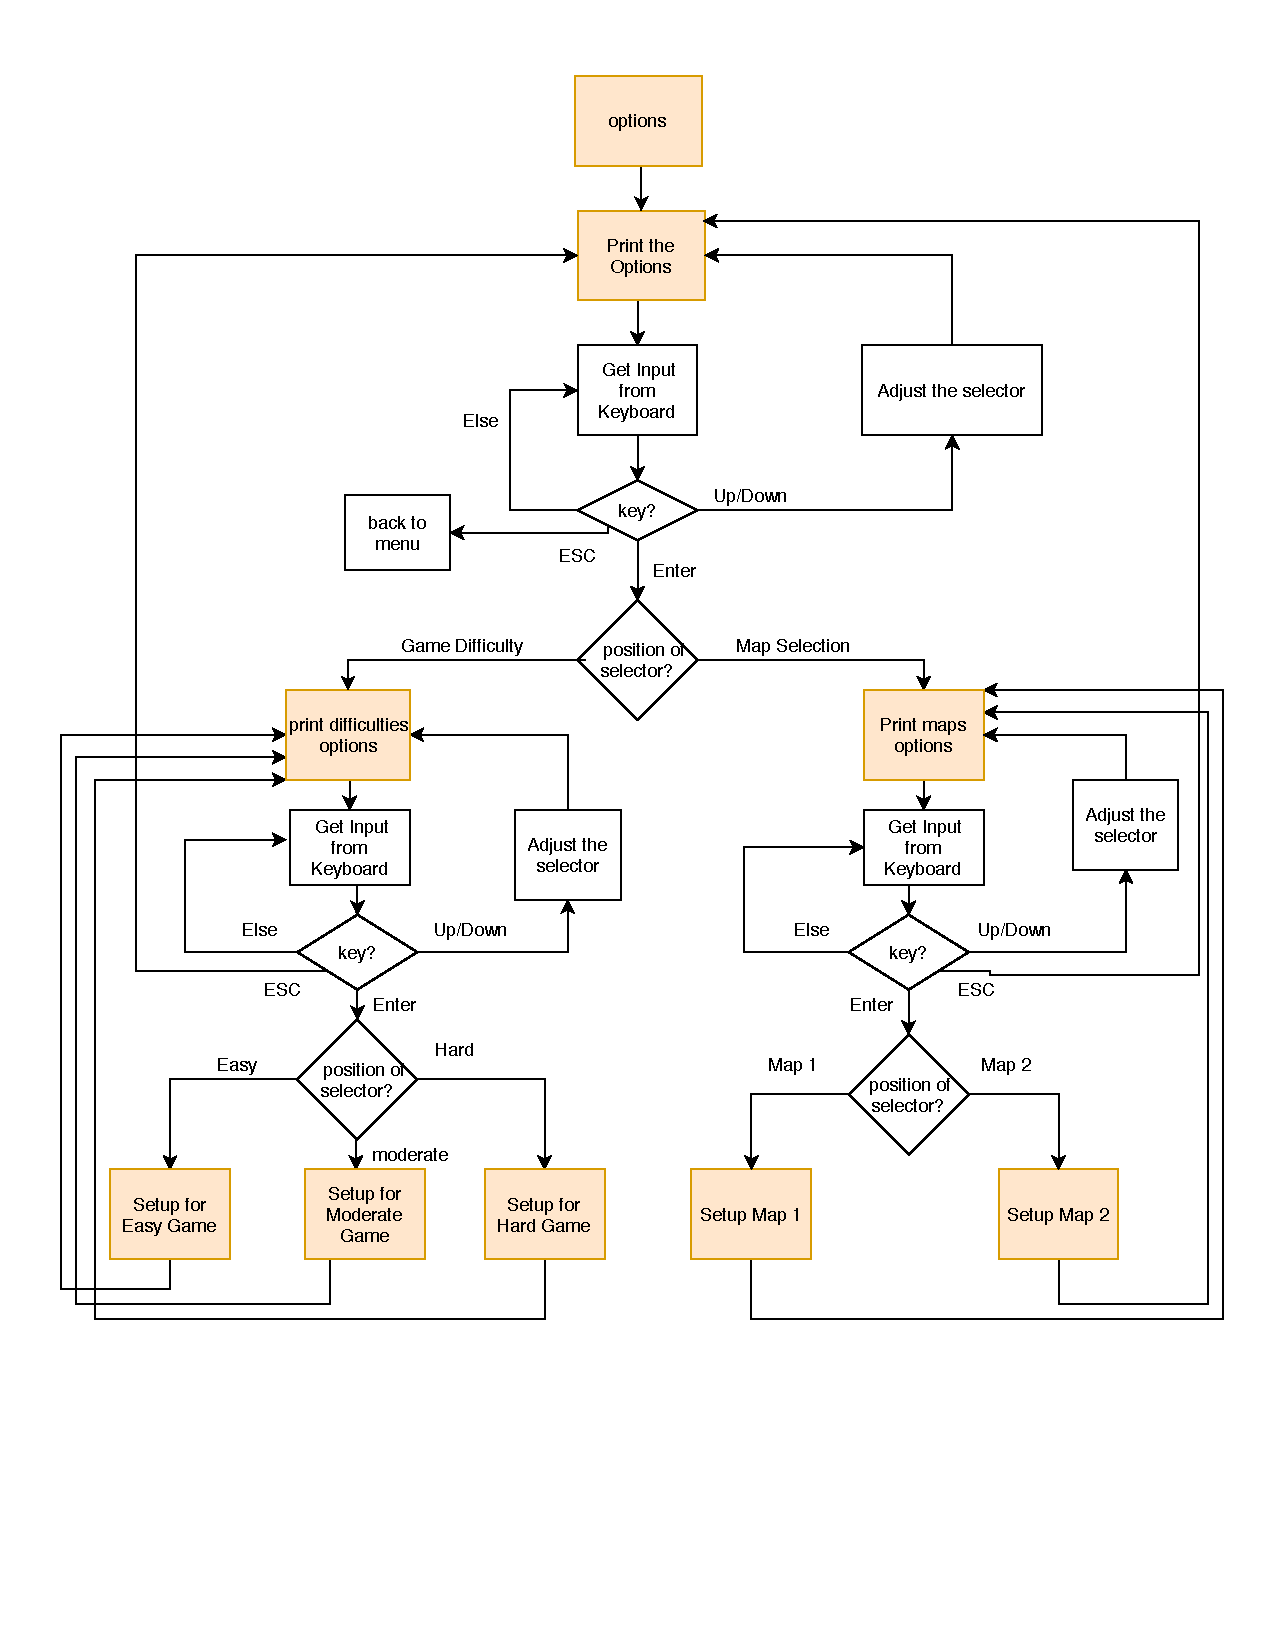
\includegraphics[width=\columnwidth]{options.pdf}
    \caption{Options block flowchart. Blocks which are in \textcolor{orange}{orange} will be implemented for the second release. Some functions and blocks are used in both menu and options which are in white color.}
    \label{fig:options}
\end{figure}

This flow chart explains all the steps happening on the options block. 
As it is shown in Figure~\ref{fig:options} initially, options items which are game difficulties are printed for the user. 
Next, according to the user input key the program goes to one of the following states: 
Enter key, Choose one difficulty level between easy, intermediate, and hard items and go back to menu.
Up/down key, go up and down between option's items.
The selected difficulty is used to do the single-player and multi-player setup later.

\subsection{Options functions prototypes}

In this section we define the required functions prototypes and its relation to flow chart~\ref{fig:options}.

\begin{minted}{c}
/**
 * @enum options_items_t
 * The enumeration of option items.
 */
typedef enum option_items{
    OPTION_ITEM_EASY,
    OPTION_ITEM_INTERMEDIATE,
    OPTION_ITEM_HARD,
    OPTION_ITEM_NUM_OF_ITEMS,
}option_items_t;

/**
 * @typedef option_t
 * A structure represents option's item.
 */
typedef struct option{
    option_items_t selector;
    item_t items[OPTION_ITEM_NUM_OF_ITEMS];
} option_t;

/**
* @brief Prints the game different difficulty options on an SDL window.
* @author Jaser
* Second release.
* @param[in] p_window A SDL window is passed to the function.
* @param[in] p_options A structure represents options item.
* @return void
*/
void print_options(SDL_Window* p_window, option_t* p_options);
\end{minted}